\documentclass[a4paper,pdftex]{article}

\usepackage{array}
\usepackage{hopsantut}

\hypersetup{pdfauthor={Robert Braun and Peter Nordin}, pdftitle={Hopsan Tutorial - Getting Started}, pdfsubject={Hopsan Tutorial}}

\begin{document}
\maketitle{Getting Started}

\section*{Introduction}
The purpose of this tutorial is to give an introduction the Hopsan simulation program, developed at the Division of Fluid and Mechatronic Systems (Flumes) at Linköping University, Sweden.
From the Hopsan GitHub project page\footnote{\url{https://github.com/Hopsan/hopsan/releases}} you can download a free version of the program.
Hopsan is available as an installation package or portable-zip version for Windows.
Deb-packages for the latest Ubuntu-distributions (a popular GNU/Linux based operating system) are also available.
If you choose the portable zip, you can try Hopsan without needing any permissions on your computer, just unzip Hopsan in a directory of your choice and then start the hopsangui.exe file from the \textit{bin} directory.

\subsection*{The Transmission Line Element Method (TLM)}
Unlike most other simulation tools Hopsan uses distributed solvers, which means that each component solves its own equations.
This has several advantages. 
First of all, it makes it possible to divide a model into smaller parts that can be simulated in parallel using multi-core processors. This can greatly reduce simulation time for large models.
Other advantages are facilitated debugging, highly robust mathematical properties and a linear relation between simulation time and model size. 
\\\\
\noindent A requirement for being able to use distributed solvers is that the modelled components can be mathematically separated from each other. 
In Hopsan the Transmission Line Element Method (TLM) is used.
By taking advantage of the natural time-delays present in real physical systems, the desired separation is achieved.
A common TLM example is a hydraulic pipe with the impedance \textbf{Zc} where the time-delay for a pressure wave through the pipe is \textbf{T}.

\begin{figure}[hbt]
  \centering
  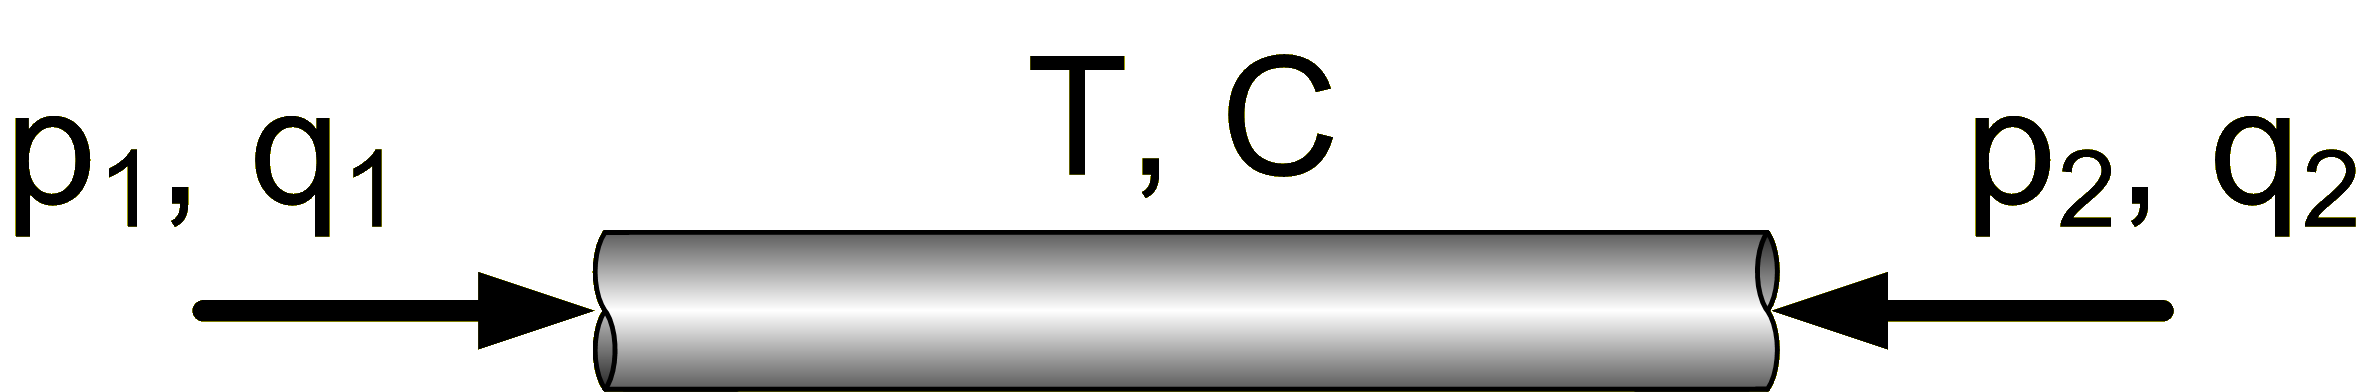
\includegraphics[width=0.6\linewidth]{gfx/PosterTransmissionLines.png}
  \caption{A hydraulic pipe can be modelled as a transmission line element}
  \label{fig:hydraulic_pipe}
\end{figure}

\noindent The pressure at one side becomes a function of the flow at that side as well as the pressure and flow at the other side \textbf{T} seconds earlier:

\begin{equation}
 p1(t) = Zc*q1(t) + p2(t-T) + Zc*q2(t_T)
\end{equation}

\noindent This means that the pressure and flow at one side of the pipe is always independent of the flow and pressure at the other side at the same time instance.
The components connected to each side of the pipe are thereby separated from each other.
In Hopsan the TLM-components, like this pipe example, are called  C-components.
Ordinary components, for example, pumps and valves, are called Q-components.

\vfill
\section*{Program Overview}
Before you build your own first Hopsan model, it is necessary to understand the different parts of the graphical user interface.
After starting Hopsan and opening a model, it will look like figure \ref{fig:hopsan_gui}.  

\begin{figure}[ht]
  \centering
  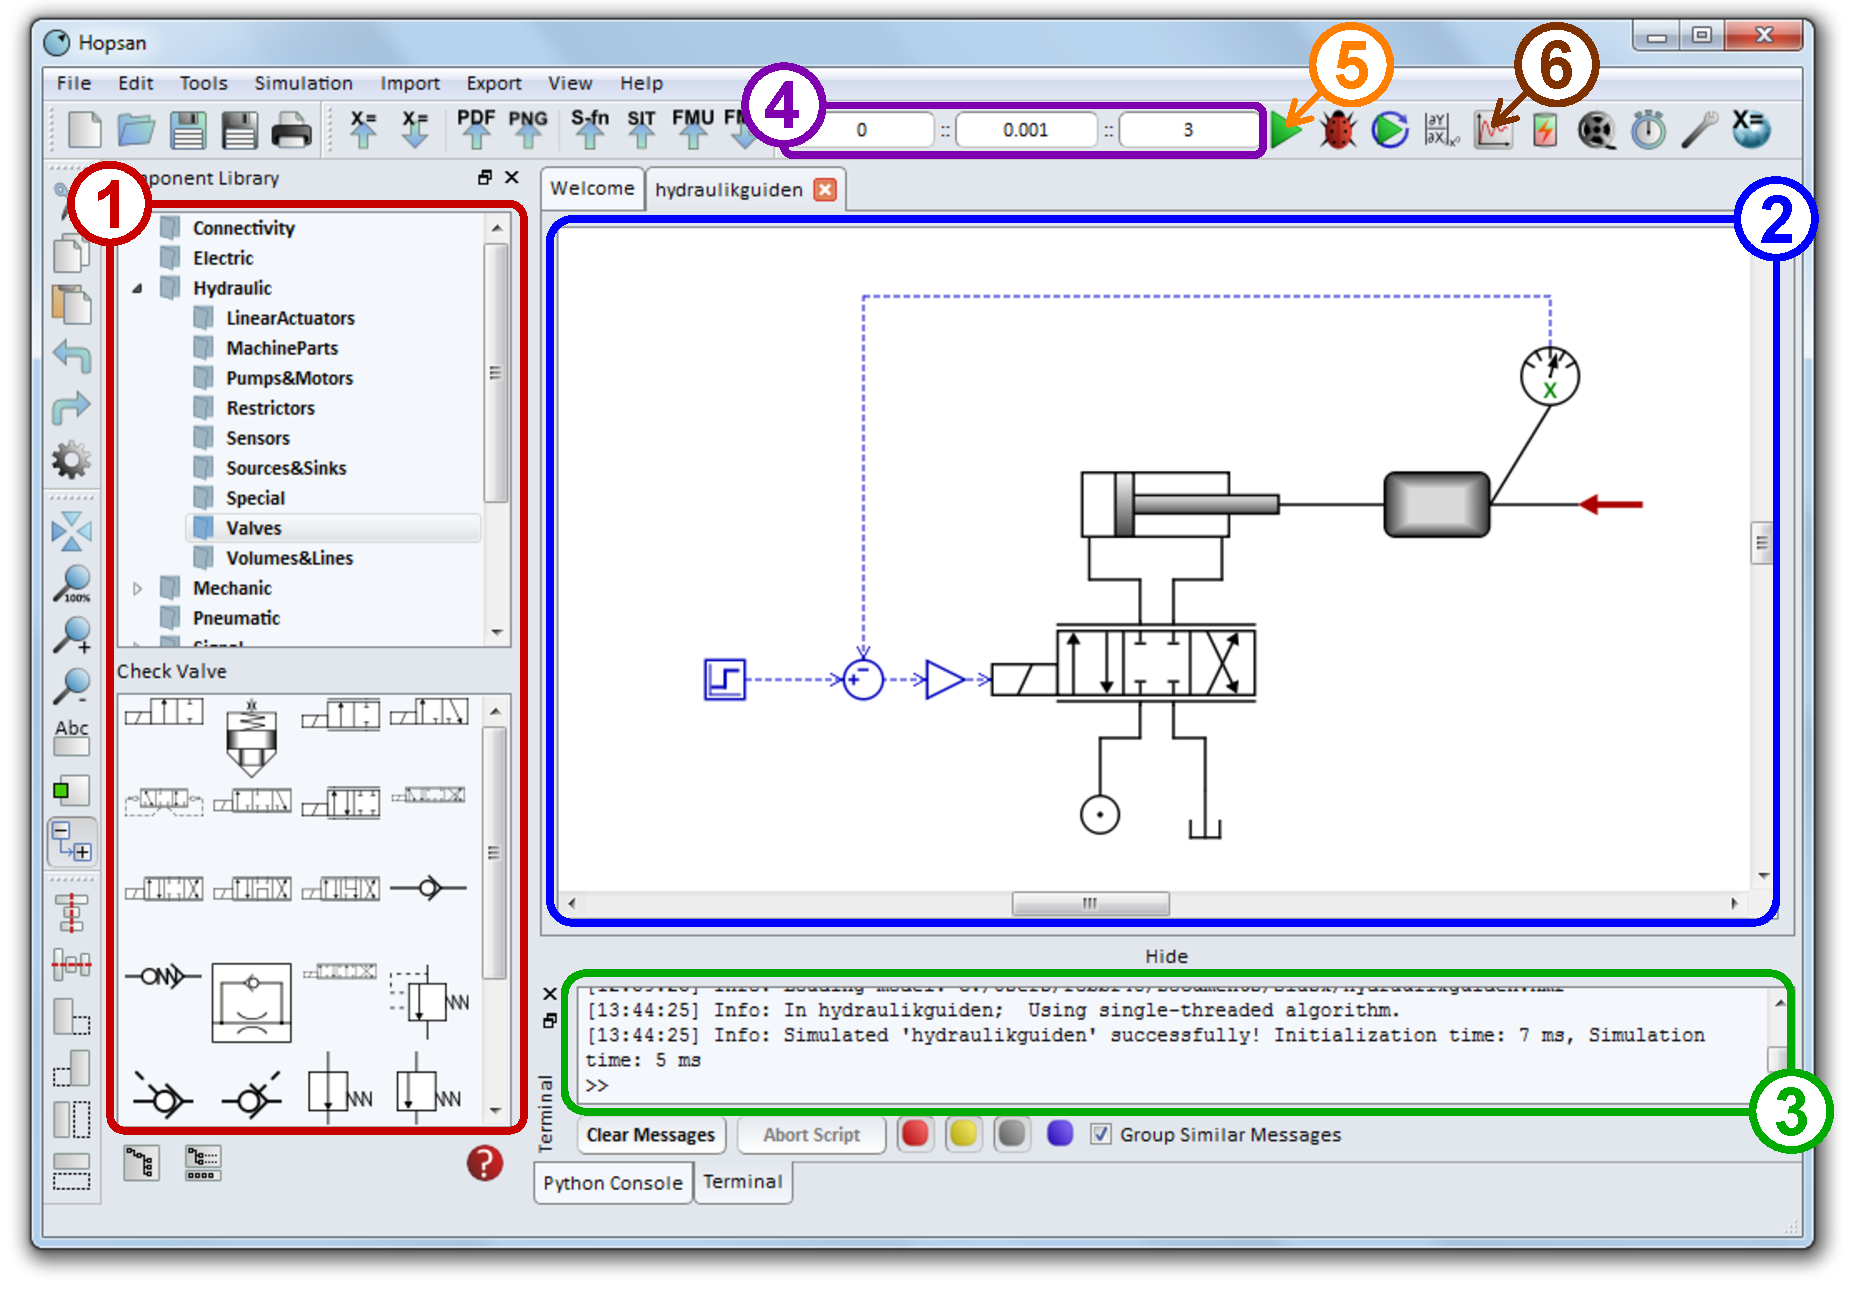
\includegraphics[width=\textwidth]{gfx/screenshot.pdf}
  \caption{The Hopsan graphical user interface}
  \label{fig:hopsan_gui}
\end{figure}

\begin{tutenumerate}
\tutitem{Component Library}
All loaded component libraries are shown here.
Components are sorted in libraries based on their relative directories.
To add a component to the model, simply drag it to the workspace and drop it.

\tutitem{Workspace}
Models are shown in the main workspace.
All added components are shown, and they can be connected as desired.
Right-clicking on a component opens a menu with various alternatives.
From here it is possible to open the Properties dialog, from where the components parameters can be modified.
This can also be accessed directly by double-clicking the component. 

\tutitem{Command terminal}
The command terminal window shows output messages from Hopsan.
These are coloured depending on their type; black for information, orange for warnings, red for errors and blue for debugging messages.
Be extra careful with the red messages, as these will often tell you when you have done something wrong.
It is also possible to give commands to Hopsan from the terminal, or to call external script files in the HCOM language.
This is, however, beyond the scope of this guide.
Write \texttt{help} in the command window for more detailed information about the available commands. 

\tutitem{Simulation time settings}
This is where the simulation start time, time step and stop time can be controlled.
It is for example possible to start the simulation before t=0, to avoid logging initial transients for a model that does not start in steady-state.
Reducing the time step will increase the accuracy of the simulation, at the cost of longer simulation time.
The number of log samples to store can be changed from the model properties dialog, accessed by the wrench icon.

\tutitem{Simulation button}
Click the green arrow button to start a simulation.
If something is wrong in your model, for example if a connection is missing, an error message will be shown in the terminal.

\tutitem{Plot button}
Click the diagram button to open a list of all logged variables from the simulation.
These can be plotted by double-clicking them, or by dragging them to the workspace.
A plot window will look like figure \ref{fig:hopsan_plotwindow}.

\begin{figure}[ht]
  \centering
  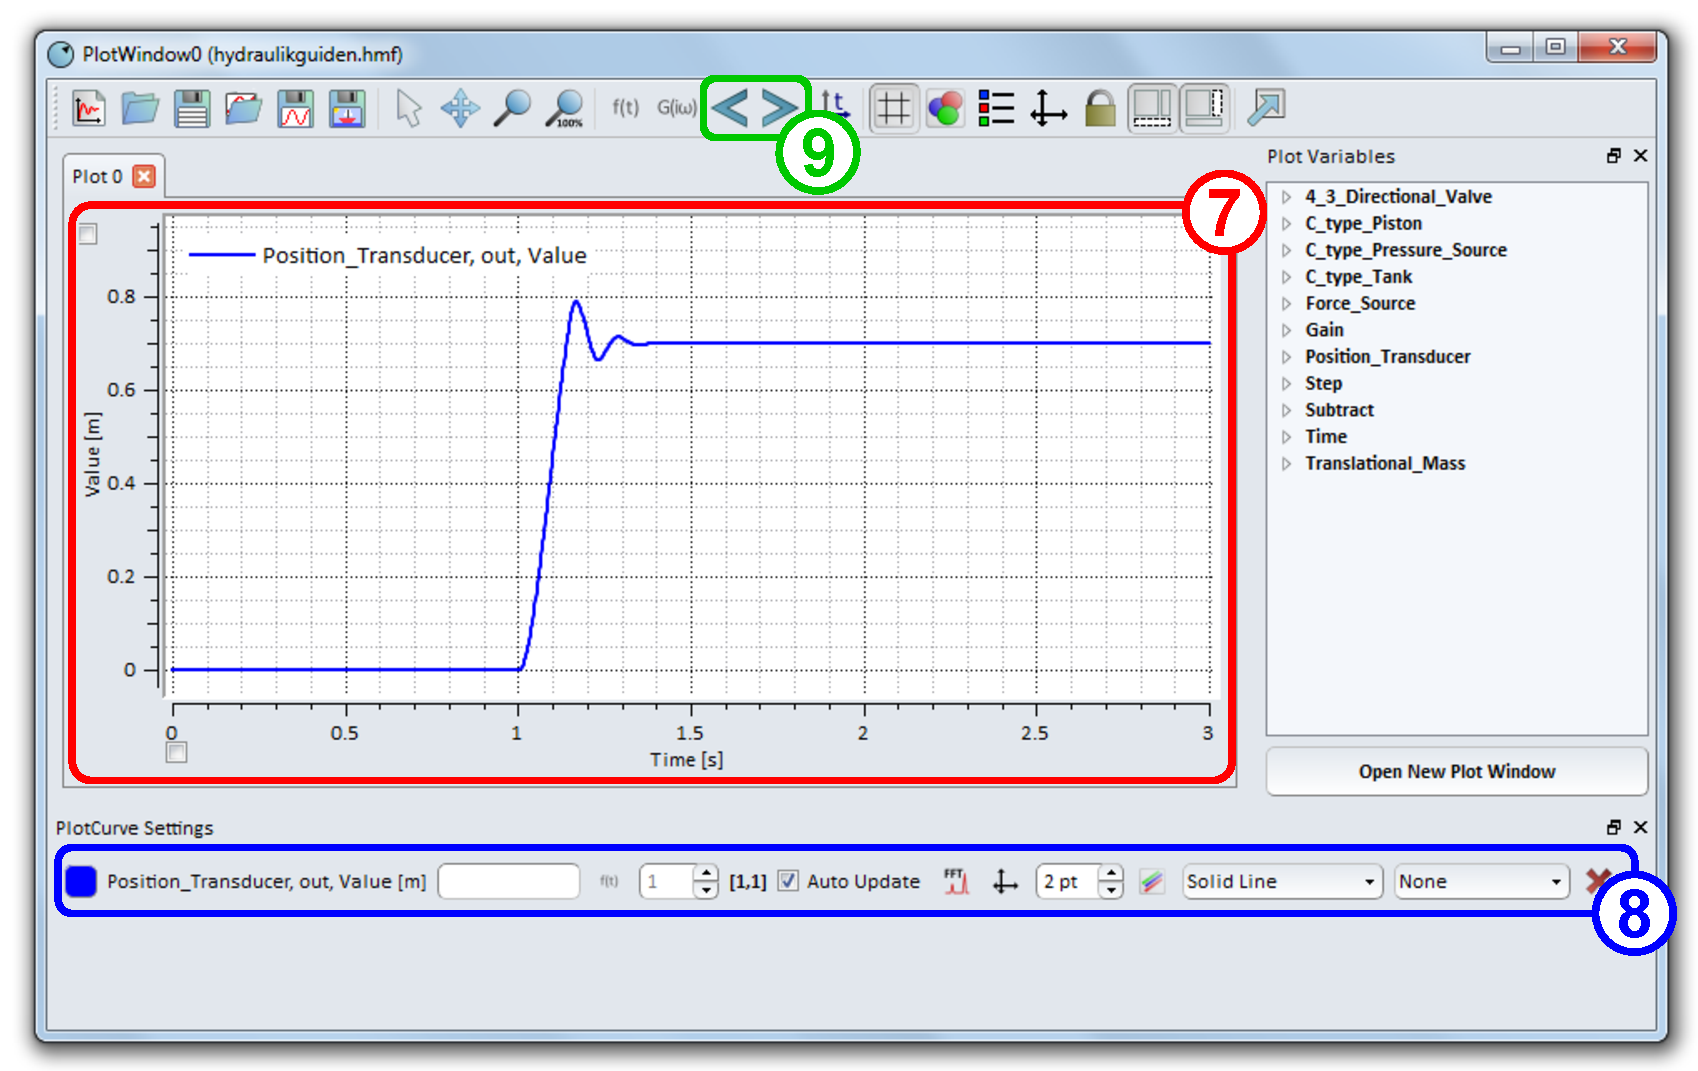
\includegraphics[width=\textwidth]{gfx/screenshot-plot.pdf}
  \caption{In the plot window the results of a simulation can be shown}
  \label{fig:hopsan_plotwindow}
\end{figure}

\tutitem{Main plot area}
Plot curves are shown here.
It is possible to add several curves to the same plot by dragging them to the left, right or bottom axes in the plot area.
Right-click in the graph for more alternatives.

\tutitem{Plot curve settings}
Appearance, generation, scaling and offset of a specific plot curve can be modified from here.
It is also possible to remove the curve with the red X icon.

\tutitem{Switch generation}
Log variables in Hopsan are grouped by generations.
After every simulation a new generation with the logged results is created.
These buttons makes it possible to increase or decrease the generation for all variables in a graph.
The generation for individual curves be can changed in the plot curve settings as described in point 8.
This makes it possible to compare the results from two different simulations, for instance after you have change parameter values in your model.
 
\end{tutenumerate}
\vfill
\section*{Building a model}
This tutorial will show how to build the model shown in Figure~\ref{fig:hopsan_gui}.
The model consists of a hydraulic position servo, where a directional valve is used to control a piston connected to a translational inertia.
A simple proportional-control feedback loop is used to position the inertia.
\begin{tutenumerate}
\tutitem{Create a new model}
Click on New Model on the welcome screen, or on the icon in the toolbar:
 	
\icon{0}{gfx/Hopsan-New.png}{Create a new empty model}
 	
\tutitem{Add components to the model}
The following components are required for the model.
A component can be found by writing its name in the Filter box, or by finding it in the library hierarchy.

\vspace{5pt}
\foldericon{0}{Hydraulic}
\foldericon{1}{Valves}
\component{2}{4/3 Directional Valve}
\foldericon{1}{Sources \& Sinks}
\component{2}{C-type Pressure Source}
\component{2}{C-type Tank}
\foldericon{1}{Linear Actuators}
\component{2}{C-type Piston}
\foldericon{0}{Mechanic}
\foldericon{1}{Linear}
\component{2}{Translational Mass}
\component{2}{Force Source}
\component{2}{Position Transducer}
\foldericon{0}{Signal}
\foldericon{1}{Source \& Sinks}
\component{2}{Step}
\foldericon{1}{Arithmetics}
\component{2}{Subtract}
\component{2}{Gain}
\vspace{5pt}

\tutitem{Connect the components}
Before you start making connections, \emph{unconnected ports} should be shown. 
You can find the button below the zoom-buttons in the left menu. 
Here you will also find a button to toggle showing the names of the components in the workspace.

\icon{0}{gfx/Hopsan-ShowPorts.png}{Show unconnected ports (Ctrl-T)}

Connections are created by clicking on the first port and finished when clicking on the second one.
Additional connection lines can be created by clicking in the workspace.
Right-clicking will remove the last created line.
\textbf{Escape} key will cancel the entire conneciton.
Hydraulic and mechanical ports are shown as green or blue squares.
Red arrows represent input and output signal ports.
Hydraulic and mechanical ports also contain the letter C or Q.
This tells you the transmission line element method (TLM) type of the component.
C-ports can only be connected to Q-ports and vice versa.
Try making an erroneous connection on purpose, and note the resulting error message.
Then connect all components according to Figure~\ref{fig:hopsan_gui}.

%\pagebreak
\vfill
\tutitem{Change parameter values}
In order to recreate the result shown in Figure~\ref{fig:hopsan_plotwindow} it is necessary to adjust some parameter values in the model.
This is done from the Properties dialog, which can be accessed by double-clicking a component.
The following parameters need to be changed:

{\renewcommand{\arraystretch}{1.2} 
\begin{tabularx}{\linewidth}{X X X}
\textbf{Component} & \textbf{Parameter} & \textbf{Value} \\
\specialrule{1.3pt}{0pt}{0pt}
C-type Pressure Source & \textit{p} & 2e7 \\
Step & \textit{y\_A} & 0.7 \\
Gain & \textit{k} & 0.015
\end{tabularx}
}

\tutitem{Simulate}
Set simulation start time, time step and stop time to 0, 0.001 and 3, respectively.
Then press the simulate button.

\icon{0}{gfx/Hopsan-Simulate.png}{Simulate current project (Ctrl-Shift-S)}

If your model is not lacking any required connections the simulation will be executed.
See the output in the terminal window for more information.

\tutitem{Plot the results}
Now plot the resulting value from the position transducer, by right-clicking on the Out-port and selecting \textit{Plot Value [m]}.
You can also use the list of log variables as described in the previous section.

\icon{0}{gfx/Hopsan-Plot.png}{Plot variables (Ctrl-Shift-P)}

Log variables can also be exported to various formats and used in other programs.
It is also possible to export the graph as a picture.

\tutitem{Change a parameter and compare the results}
Now change the parameter \textbf{k} in the component \textbf{Gain} to \textbf{0.03}, i.e. twice as high as before.
Simulate again and go back to the plot window and change generation to compare the curves.
It is also possible to add the same curve twice and see the two generations in the same graph.

\tutitem{Animation}
Sometimes it is difficult to understand a system by just looking at the graphs.
In the toolbar at the top, there is a button that starts the animation function.
Click that button!

\icon{0}{gfx/Hopsan-Animation.png}{Animate}

This opens the animation mode.
There is a new special toolbar that controls the animation.
Click at the \textit{Play} icon to start a replay animation of the system you just simulated. 

\icon{0}{gfx/Hopsan-Play.png}{Start replay animation}

You can also click on \textit{Play interactive animation} icon to start a real-time animation where the model is simulated during animation.

\icon{0}{gfx/Hopsan-PlayRealTime.png}{Start interactive animation}

Return to the model by clicking the red X icon at the right end of the toolbar.
\end{tutenumerate}

\end{document}